\section{The \tSS{} and validation}
This section describes the \tSS{} that
has been inserted in the testsuite folder of the library. It shows the
numerical validation that has been carried out in order to ensure that
the numerical solver works properly.

The \tSS{} implements the steady case of homogeneous pure strain of a
cube. The problem reads as follows:
\begin{equation} \left\{
    \begin{array}{lllllll} \displaystyle \text{Div}(\Piola) +
      \rho_0\underline{b} = \underline{0} & \text{on} \quad [0,L]^3,\\ \\
      \displL(t)=\underline{0} & \text{on} \quad \Gamma_D, \quad t>0,\\
      \Piola\underline{n}_2=\underline{t}_0 & \text{on} \quad \Gamma_{N_2},
      \quad t>0.\\
    \end{array}\right.
  \label{eq::homStrain}
\end{equation}
where $L$ is the length of the cube
side. Fig.~\ref{fig::pureStrain} is the two dimensional representation
of \eqref{eq::homStrain}. As represented in the figure, the applied
stress has only nonzero component along the axis perpendicular to the
surface.
\begin{figure} \centering
  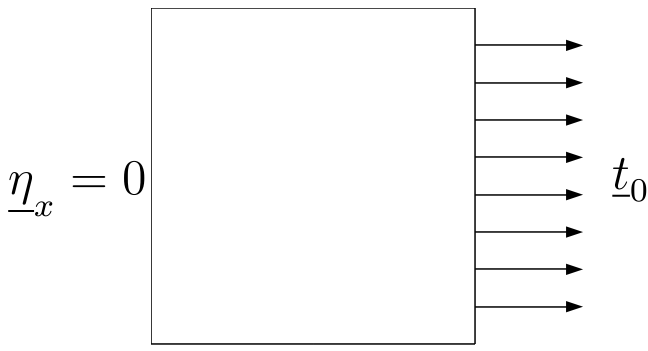
\includegraphics[width=0.35\textwidth]{images/modelProblem.png}
  \caption{2D representation of Problem \eqref{eq::homStrain}}
  \label{fig::pureStrain}
\end{figure}
\begin{figure} \centering
  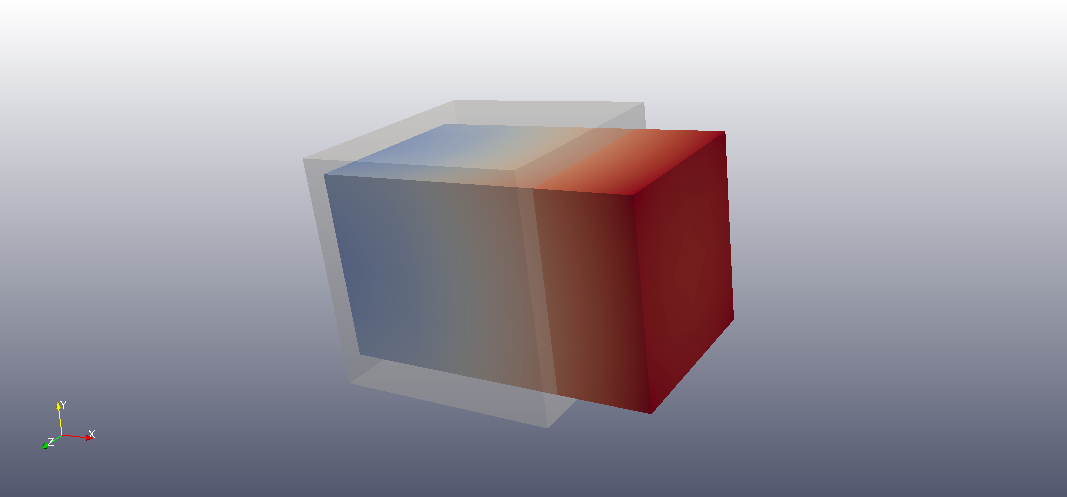
\includegraphics[width=0.45\textwidth]{images/cube_exp_timeAdvance-BDF1.png}
  \caption{Deformation of the cube under the applied traction}
  \label{fig:displ}
\end{figure}

Fig.\ref{fig:displ} shows the deformation of the cube under the
applied traction. The simple model problem \eqref{eq::homStrain}
allows to find an analytical expression of the first Piola-Kirchhoff
tensor. In this case, the deformation gradient \F{} and the right
Cauchy-Green tensor \C{} read
\begin{equation} \F = \left(
    \begin{array}{ccc} \lambda_1 & 0 & 0 \\ 0 & \lambda_2 & 0 \\ 0 & 0 &
      \lambda_3
    \end{array}\right)\qquad\quad \C = \left(
    \begin{array}{ccc} \lambda_1^2 & 0 & 0 \\ 0 & \lambda_2^2 & 0 \\ 0 &
      0 & \lambda_3^2
    \end{array}\right)
\end{equation}
In this case, the invariants of \C{} depend only on the
deformations $\lambda_i$. Consequently, according to
\eqref{eq::WandInvariants} the function \W{} depends on the diagonal
elements of \F{}. Moreover, \W{} satisfy the simmetries
\begin{equation}
  \WE(\lambda_1,\lambda_2,\lambda_3)=\WE(\lambda_1,\lambda_2,\lambda_3) =
  \WE(\lambda_1,\lambda_3,\lambda_2)=\WE(\lambda_3,\lambda_1,\lambda_2).
  \label{eq::W&Lambda}
\end{equation}
Furthermore, due to the simmetry of the test case,
$\lambda_2=\lambda_3$ and they can be derived by the determinant of \F{}
thanks to the relation
\begin{equation} \displaystyle
  \lambda_2=\lambda_3=\sqrt{\frac{J}{\lambda_1}},
  \label{eq::diffLambda}
\end{equation}
where $J=\text{det}\F$. Inserting
\eqref{eq::diffLambda} in \eqref{eq::W&Lambda}, the general form of \W{}
becomes
\begin{equation} \displaystyle
  \WE=\WE(\lambda_1,\sqrt{\frac{J}{\lambda_1}}\big).
  \label{eq::syntW}
\end{equation}
Thanks to \eqref{eq::syntW}, it is possible to compute
the first Piola-Kirchhoff tensor analitically. In particular, the
exact expression of the term $\Piola_{11}$ can be deduced. Since the
determinant $J$ is present in \eqref{eq::syntW}, we consider also the
term $\Piola_{22}$. In the following, the expression of $\Piola_{11}$
for the three constitutive laws is provided:
\begin{itemize}
\item \textit{St. Venant-Kirchhoff}:
  \begin{equation}
    \begin{array}{lll} & \Piola_{11}=\displaystyle
      \frac{\lambda}{2}(I_{\C}-3)\lambda_1 - \mu\lambda_1 +
      \mu\lambda_1^3;\\ \\ & \Piola_{22}=\displaystyle
      \frac{\lambda}{2}(I_{\C}-3)\lambda_2 - \mu\lambda_2 + \mu\lambda_2^3;
    \end{array}
    \label{eq::P11SVK}
  \end{equation}
\item \textit{Neo-Hookean}:
  \begin{equation}
    \begin{array}{lll} & \Piola_{11}=\displaystyle \mu J^{-2/3}
      (\lambda_1 - \frac{I_{\C}}{3\lambda_1}) + \frac{\kappa}{2}(J^2 - J +
      log(J))\frac{1}{\lambda_1};\\ \\ & \Piola_{22}=\displaystyle \mu
      J^{-2/3} (\lambda_1 - \frac{I_{\C}}{3\lambda_2}) +
      \frac{\kappa}{2}(J^2 - J + log(J))\frac{1}{\lambda_2};
    \end{array}
    \label{eq::P11NH}
  \end{equation}
\item \textit{Exponential}:
  \begin{equation}
    \begin{array}{lll} & \Piola_{11}=\displaystyle \alpha \term
      J^{-2/3}(\lambda_1 - \frac{I_{\C}}{3\lambda_1})+\frac{\kappa}{2}(J^2 -
      J + log(J))\frac{1}{\lambda_1};\\ \\ & \Piola_{22}=\displaystyle
      \alpha \term J^{-2/3}(\lambda_2 -
      \frac{I_{\C}}{3\lambda_2})+\frac{\kappa}{2}(J^2 - J +
      log(J))\frac{1}{\lambda_2};
    \end{array}
    \label{eq::P11EXP}
  \end{equation}
\end{itemize}
The procedure that has been followed is the following:
\begin{enumerate}
\item a specific traction is applied on the Neumann face of the cube
  and the deformation $\lambda_1$ is obtained numerically;
\item the term $\Piola_{22}$ is equal to zero and then, the
  expression of $J$ as a function of $\lambda_1$ can be computed.
\item the function $J=J(\lambda_1)$ is introduced in one of the
  three expressions of $\Piola_{11}$ according to the chosen
  constitutive law and the value of $\Piola_{11}$ deduced. If the code
  works properly, the value of $\Piola_{11}$ using the computed
  deformation is equal to the applied traction.
\end{enumerate}
The numerical test has been carried out on a
structured mesh of 125 nodes. The polynomial space is P1. The material
parameters are the following:
\begin{itemize}
\item \textit{Poisson ratio} $= 0.45$;
\item \textit{Young modulus} $= 6e6$;
\item $\kappa$ $=1e8$;
\item $\alpha$ $=2e6$;
\item $\gamma$ $=0.80$;
\end{itemize}
After having obtained the deformation $\lambda_1$ and
computed the corresponding term in \Piola{}, the relative error
\begin{equation} err = \displaystyle
  \frac{\Piola_{11-analitical}-\Piola_{11-numerical}}{\Piola_{11-analitical}},
\end{equation}
where $\Piola_{11-analitical}$ is the applied traction
force and $\Piola_{11-numerical}$ is the stress computed using the
procedure explained above, has been analyzed.

Figs.\ref{fig:errLE},\ref{fig:errSVK},\ref{fig:errNH},\ref{fig:errEXP}
show the comparisons between the analytical and numerical relation
between $\Piola_{11}$ and the behaviour of the relative error when
different loads are applied and, consequently, different deformations
are obatined.

\begin{figure}[h!]
  \centering
  \subfigure[Stress-Strain relation]{
    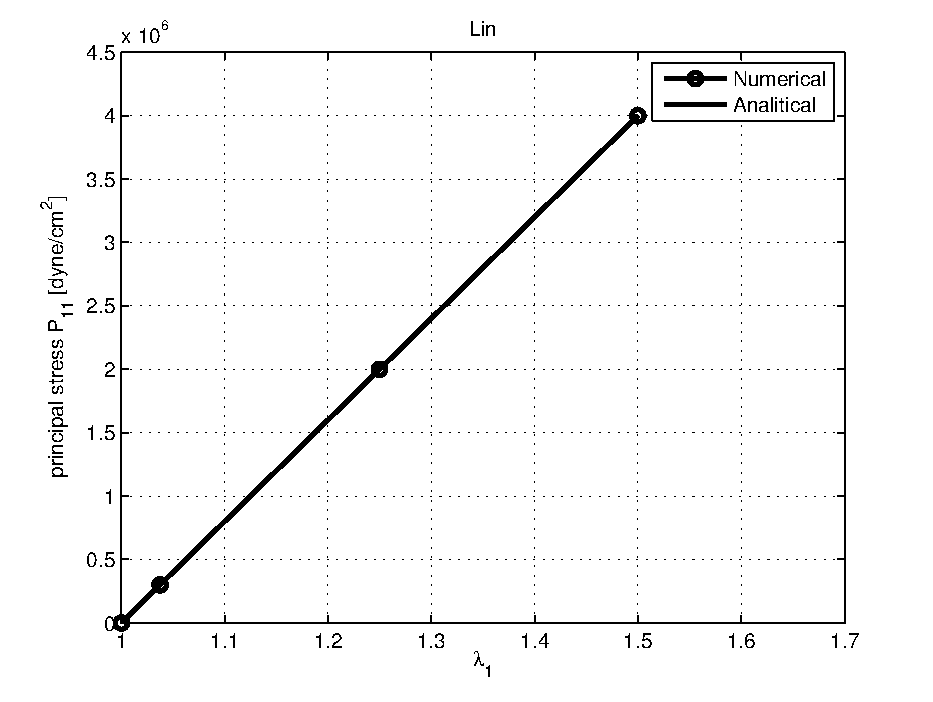
\includegraphics[width=0.32\textwidth]{images/sigepsP1-Lin-BDF1.pdf}}
  \subfigure[Relative error]{
    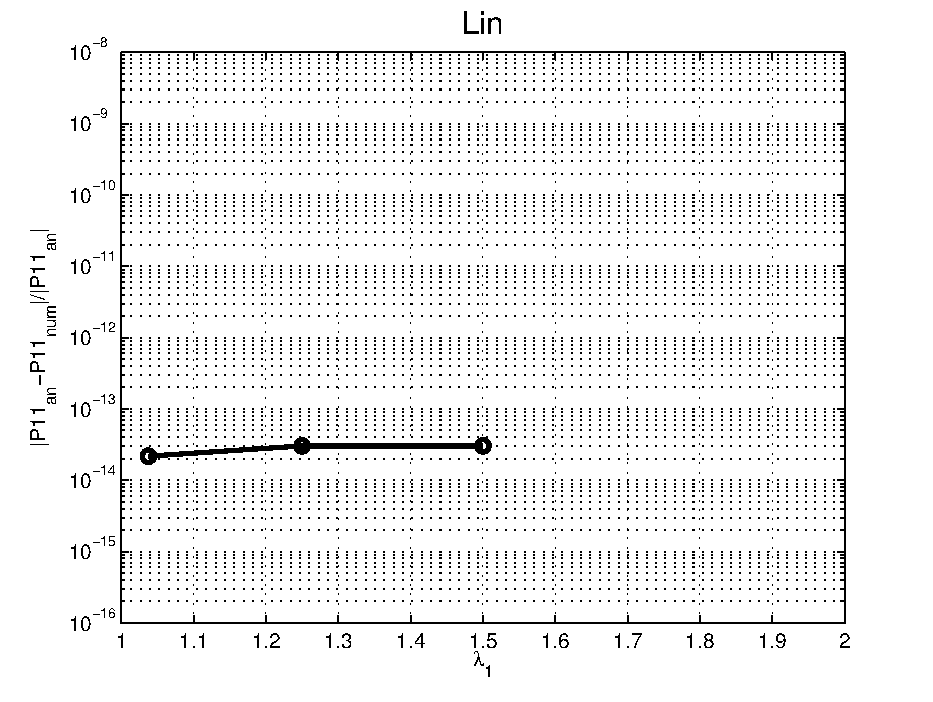
\includegraphics[width=0.32\textwidth]{images/errorP1-Lin-BDF1.pdf}}
  \caption{Comparison between analytical and numerical solution for
    Linear Elastic}
  \label{fig:errLE}
\end{figure}

\begin{figure}[h!]
  \centering
  \subfigure[Stress-Strain relation]{
    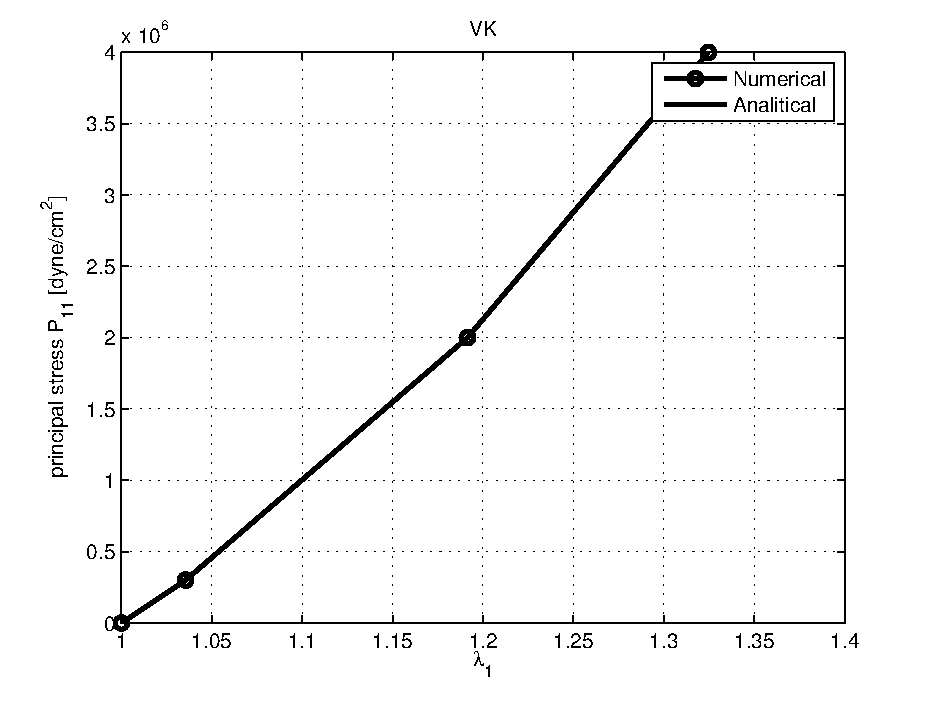
\includegraphics[width=0.32\textwidth]{images/sigepsP1-SVK-BDF1.pdf}}
  \subfigure[Relative error]{
    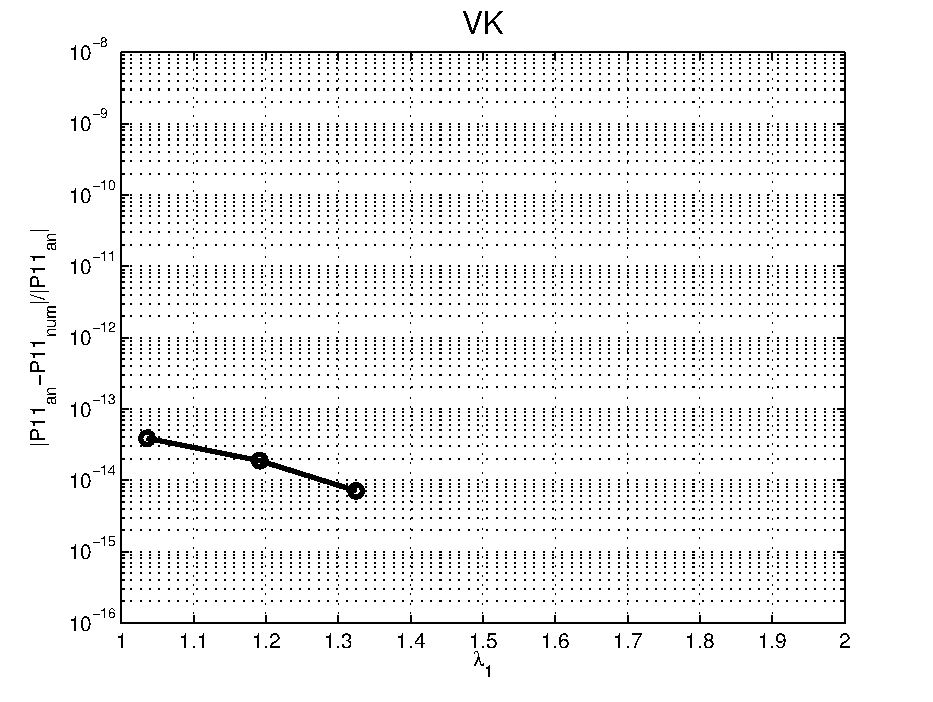
\includegraphics[width=0.32\textwidth]{images/errorP1-SVK-BDF1.pdf}}
  \caption{Comparison between analytical and numerical solution for
    St. Venant-Kirchhoff}
  \label{fig:errSVK}
\end{figure}

\begin{figure}[h!]
  \centering
  \subfigure[Stress-Strain relation]{
    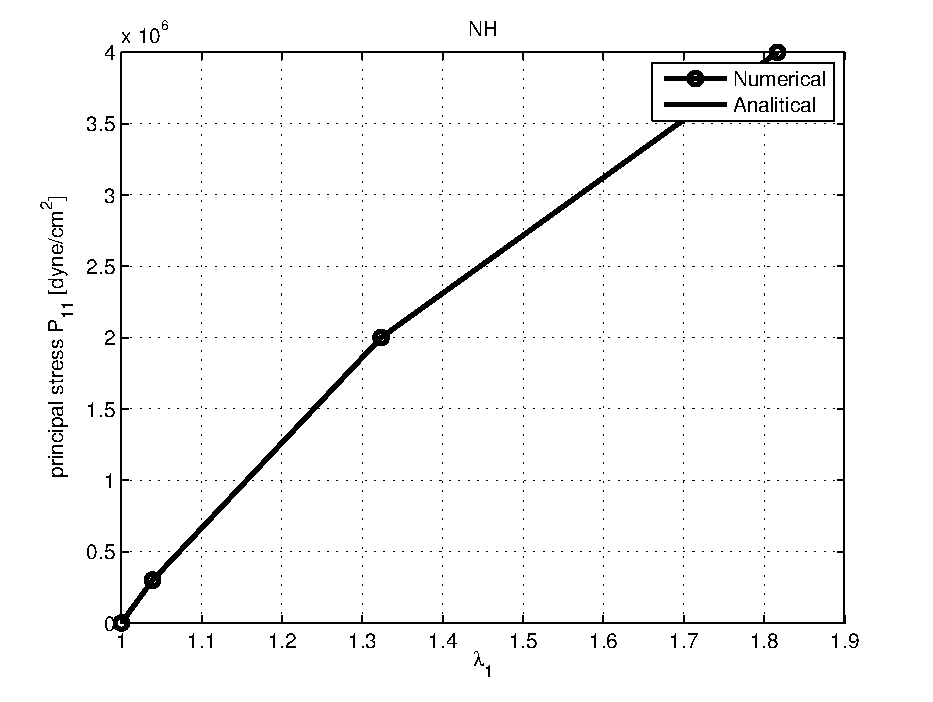
\includegraphics[width=0.32\textwidth]{images/sigepsP1-NH-BDF1.pdf}}
  \subfigure[Relative error]{
    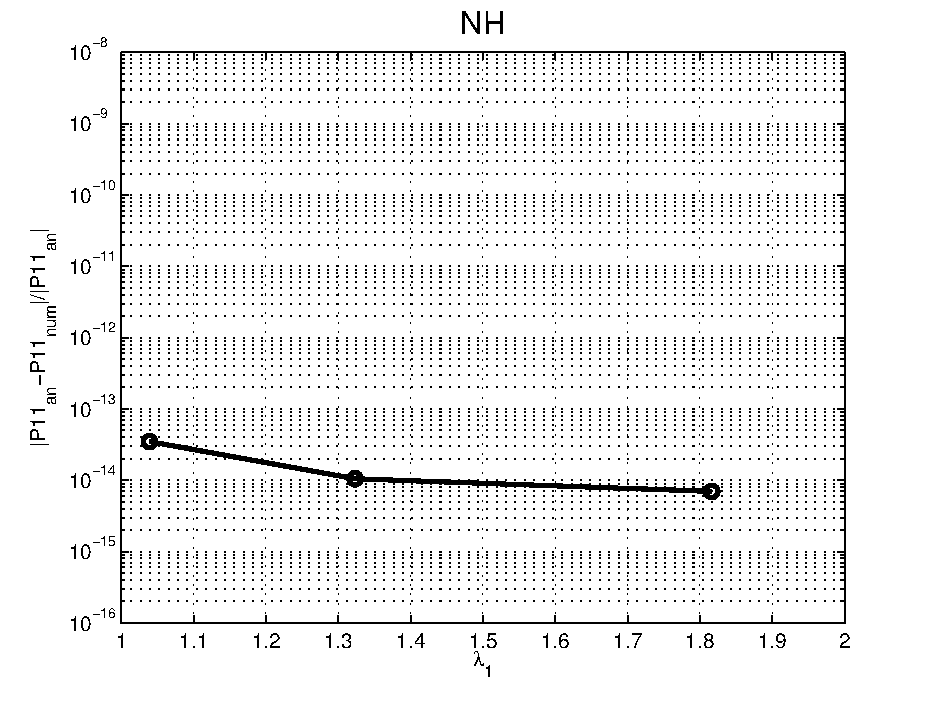
\includegraphics[width=0.32\textwidth]{images/errorP1-NH-BDF1.pdf}}
  \caption{Comparison between analytical and numerical solution for
    Neo-Hookean}
  \label{fig:errNH}
\end{figure}

\begin{figure}[h!]
  \centering
  \subfigure[Stress-Strain relation]{
    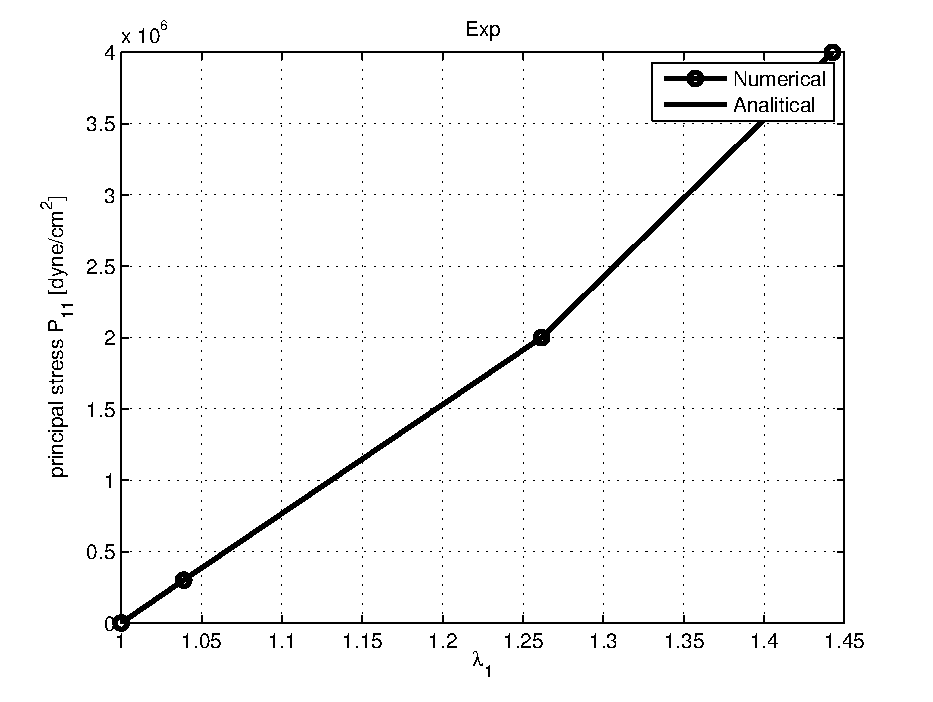
\includegraphics[width=0.32\textwidth]{images/sigepsP1-EXP-BDF1.pdf}}
  \subfigure[Relative error]{
    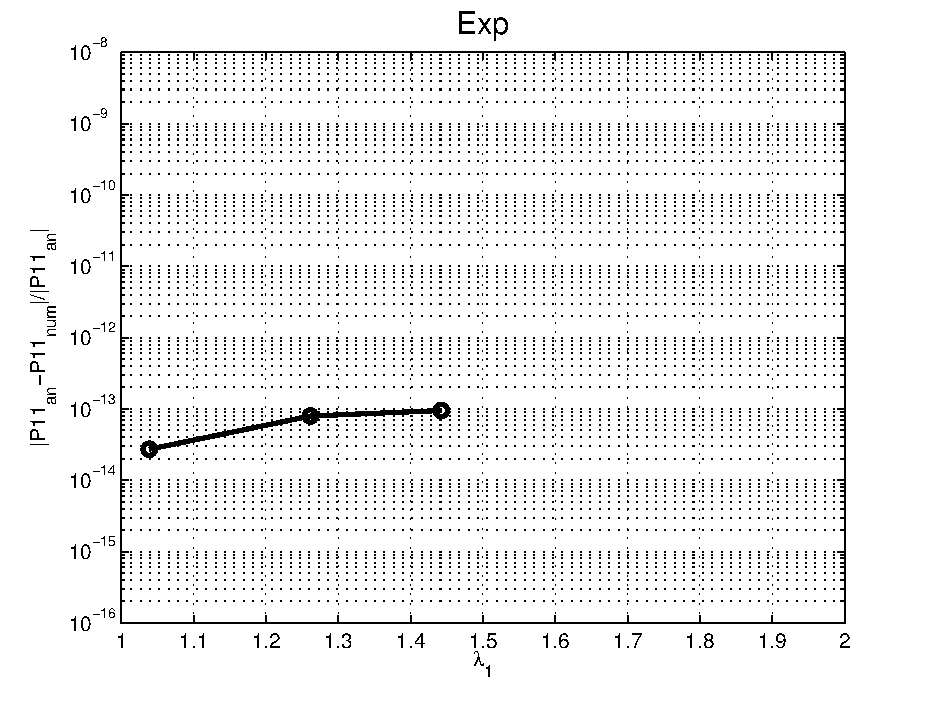
\includegraphics[width=0.32\textwidth]{images/errorP1-EXP-BDF1.pdf}}
  \caption{Comparison between analytical and numerical solution for
    exponential}
  \label{fig:errEXP}
\end{figure}

